\section{Artículo principal}
\label{articulo_principal}

\comment{Aquí se habla del artículo principal\\}

El artículo principal, \textit{A Note on ``Solving the Find-Path Problem by Good Representation of Free Space''}, es una crítica a un artículo de Brooks, llamado \textit{Solving the Find-Path Problem by Good Representation of Free Space}. En esta sección se llevará a cabo una introducción al artículo original de Brooks, explicando los puntos principales. Posteriormente, se explicarán las críticas que el artículo principal realiza sobre el artículo de Brooks.

\subsection{Solving the Find-Path Problem by Good Representation of Free Space}

El método que Brooks expone en este artículo se basa en la representación del espacio libre como conos generalizados. Un cono geralizado es un cono truncado que tiene una base y una tapa formada por cilindros (figura \ref{fig:cono_generalizado}).\\

\begin{figure}[h]
		\centering
        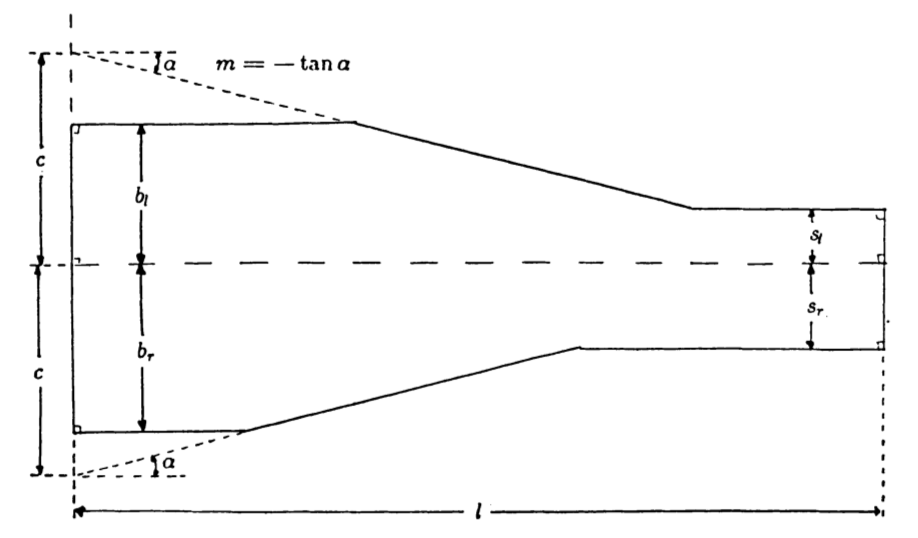
\includegraphics[width=0.35\textwidth]{images/cono_gen.png}
        \caption{Cono generalizado en un plano 2D}
        \label{fig:cono_generalizado}
\end{figure} 

El algoritmo propuesto es el siguiente. Primero, el mapa del entorno es analizado, y se calculan los conos generalizados que proporcionarán las trajectorias sin colisión. Este paso puede ser realizado en un tiempo $O(n^3)$. A continuación se procesan estos conos por parejas, comprobando para cuáles de ellos existe intersección entre sus columnas. La columna del cono generalizado es el eje de revolución del mismo. Hasta este punto, el algoritmo es independiente del objeto que se deseee mover por el entorno y, por tanto, sólo es necesario ejecutar esta parte del algoritmo una vez por cada entorno (suponiendo que el entorno es estático).\\

Cada intersección debe ser comprobada y anotada con el rango angular que describe las orientaciones del objeto en las que está garantizado que ese objeto quede contenido dentro del cono generalizado. De esta forma, se especifican las orientaciones o rotaciones permitidas para el objeto en cada una de las intersecciones.\\

Finalmente, se genera el grafo que contiene todas las rutas posibles, comprobando que, para cada intersección, el ángulo requerido para viajar de una intersección a la siguiente está contenido dentro del rango calculado en el paso anterior. Este grafo nos daría todas los caminos libres de colisión que existen en el entorno, asegurándonos que si viajamos desde un nodo A a un nodo B de este grafo con nuestro objeto no existirá colisión con ningún obstáculo. El hecho de usar las columnas de los conos generalizados nos grantiza también que el objeto recorrerá el camino lo más alejado posible de los obstáculos.\\

Una vez tenemos el grafo, se puede realizar la búsqueda del camino más corto de un nodo a otro del grafo usando un algoritmo de búsqueda en grafos tal como el $A^*$. El camino resultante será un conjunto de tramos rectos en los que el objeto se desplará usando translaciones puras y un conjunto de nodos en los que el objeto se reorientará mediante rotaciones puras para dirigirse al siguiente nodo.\\

El método para generar los conos generalizados está ampliamente detallado en el artículo, \comment{y un resumen sería bla, bla, bla}.\\

\subsection{A Note on ``Solving the Find-Path Problem by Good Representation of Free Space''}

\newpage

